\documentclass[11pt]{article}

\usepackage[margin=0.8in]{geometry}

\usepackage{graphicx}

\usepackage{booktabs}

\usepackage{float}

\usepackage{hyperref}

\usepackage{xcolor}

\graphicspath{{./}}

\title{Nonrephasing Controls for the SOC Bright--Dark Model}

\author{LiouvilleSolver SOC model notes}

\date{\today}

\begin{document}

\maketitle

\section{Purpose}

This document compares the existing rephasing and nonrephasing third-order 1Q spectra for the four priority SOC-model tests.  No new spectra were calculated here; the analysis reads the saved \texttt{S\_data.npz} files and extracts finite-window observables.

The spectral maps below use independent colour normalisation for each panel.  The quantitative amplitude comparison is therefore given by the tables, not by the visual colour scale.

For the spectral maps, rephasing is shown in the conventional $(-\omega_1,+\omega_3)$ quadrant, while nonrephasing is shown in the $(+\omega_1,+\omega_3)$ quadrant.  The displayed maps use zoom spectra evaluated on a narrow window around the bright feature.

\section{Validation summary}

\begin{itemize}

\item Corrected spectra place rephasing in the (-omega1,+omega3) quadrant and nonrephasing in the (+omega1,+omega3) quadrant.

\item The nonrephasing peak is centered at positive omega1 for every displayed case.

\item The corrected zoom-window amplitudes are comparable to the rephasing amplitudes in this symmetric model.

\item The earlier broad-grid nonrephasing ratios should not be used for amplitude conclusions because they sampled omega1 < 0.

\end{itemize}

\section{Step 6: dynamic phonon parameter scans}

The nonrephasing channel tests whether the redistribution with $g_Q$ and $\omega_Q$ survives a different time ordering.

\begin{table}[H]

\centering

\begin{tabular}{lrrrr}
\toprule
Case & max NR/R & $||S_{NR}||/||S_R||$ & area NR/R & NR peak $\omega_1$ \\
\midrule
gQ\_0 & 1.018 & 1.018 & 1.018 & 1.004 \\
gQ\_0p01 & 1.037 & 1.041 & 1.048 & 1.005 \\
omegaQ\_0p07 & 1.051 & 1.054 & 1.073 & 1.006 \\
\bottomrule
\end{tabular}

\caption{Finite-window nonrephasing ratios for Step 6: dynamic phonon parameter scans.}

\end{table}

\begin{figure}[H]

\centering

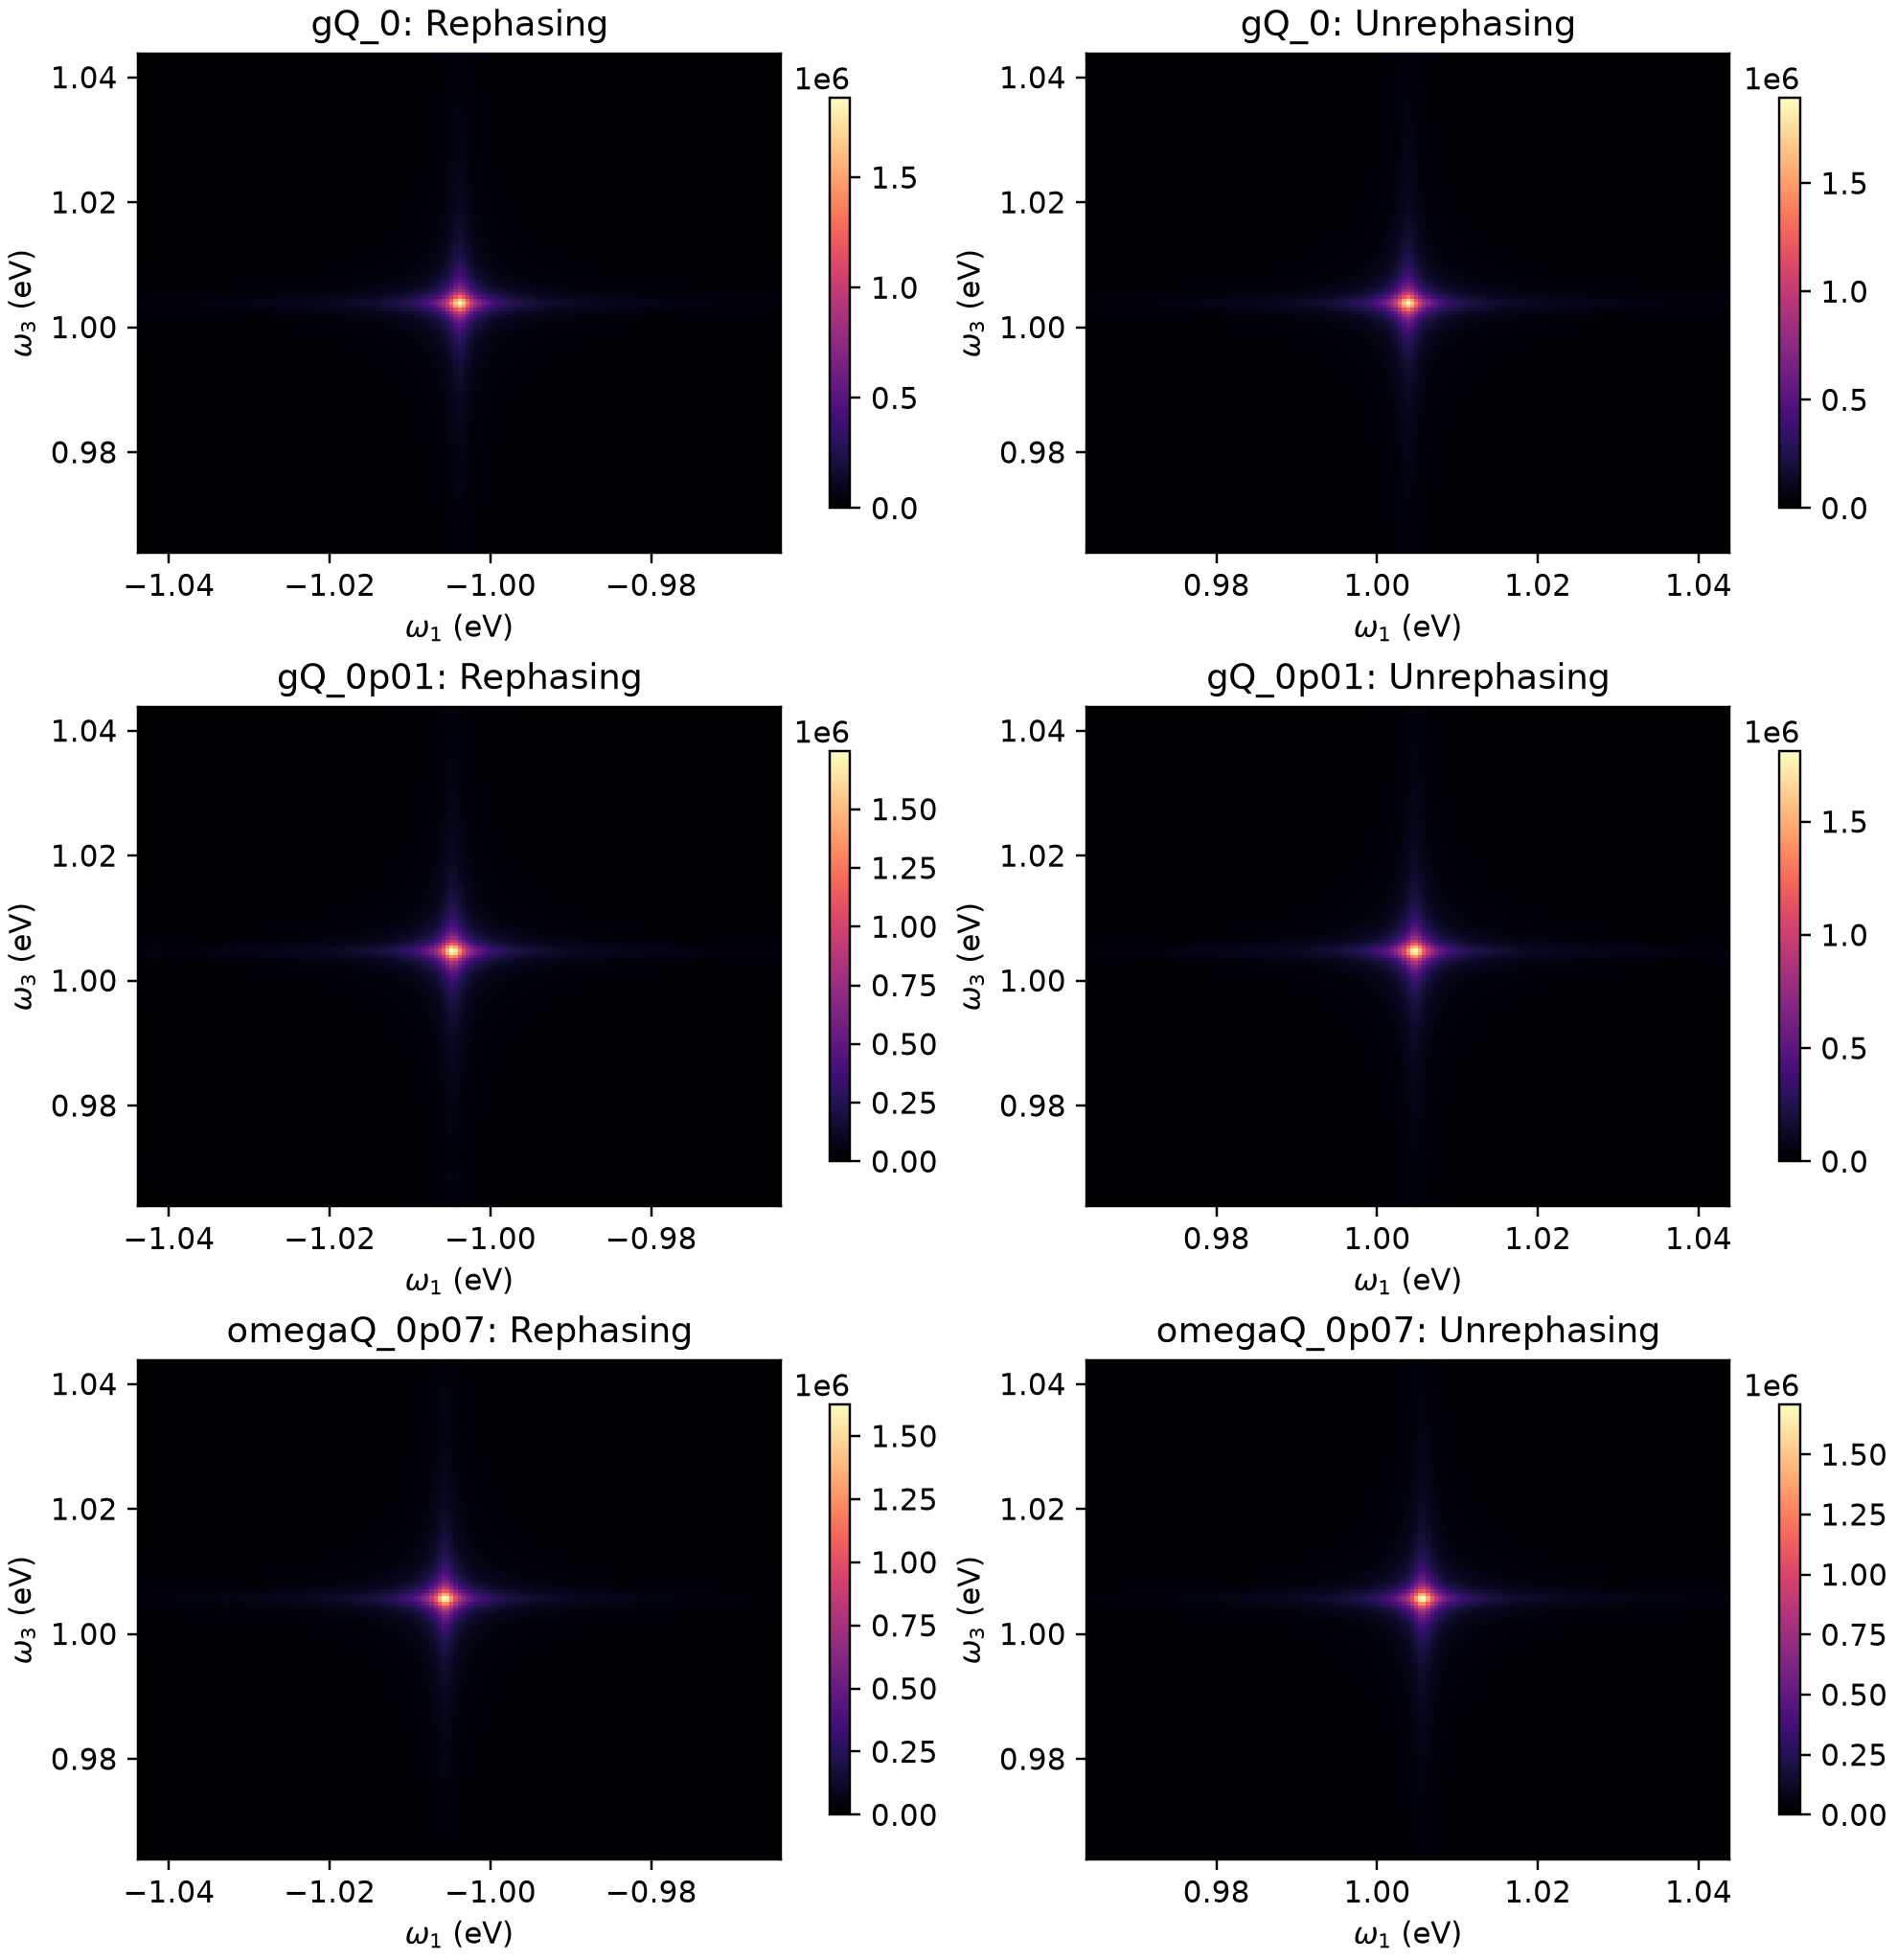
\includegraphics[width=0.98\linewidth]{spectra_etape_6_rephasing_unrephasing_abs.png}

\caption{Representative $|S|$ spectra. Left column: rephasing; right column: nonrephasing. Each panel is independently normalised.}

\end{figure}

\section{Step 3: static controls versus dynamic phonon}

The key check is whether the two static controls remain degenerate while the dynamic phonon case becomes distinct.

\begin{table}[H]

\centering

\begin{tabular}{lrrrr}
\toprule
Case & max NR/R & $||S_{NR}||/||S_R||$ & area NR/R & NR peak $\omega_1$ \\
\midrule
static\_dimerisation & 1.018 & 1.018 & 1.018 & 1.004 \\
dynamic\_dimerisation\_phonon & 1.037 & 1.041 & 1.048 & 1.005 \\
\bottomrule
\end{tabular}

\caption{Finite-window nonrephasing ratios for Step 3: static controls versus dynamic phonon.}

\end{table}

\begin{figure}[H]

\centering

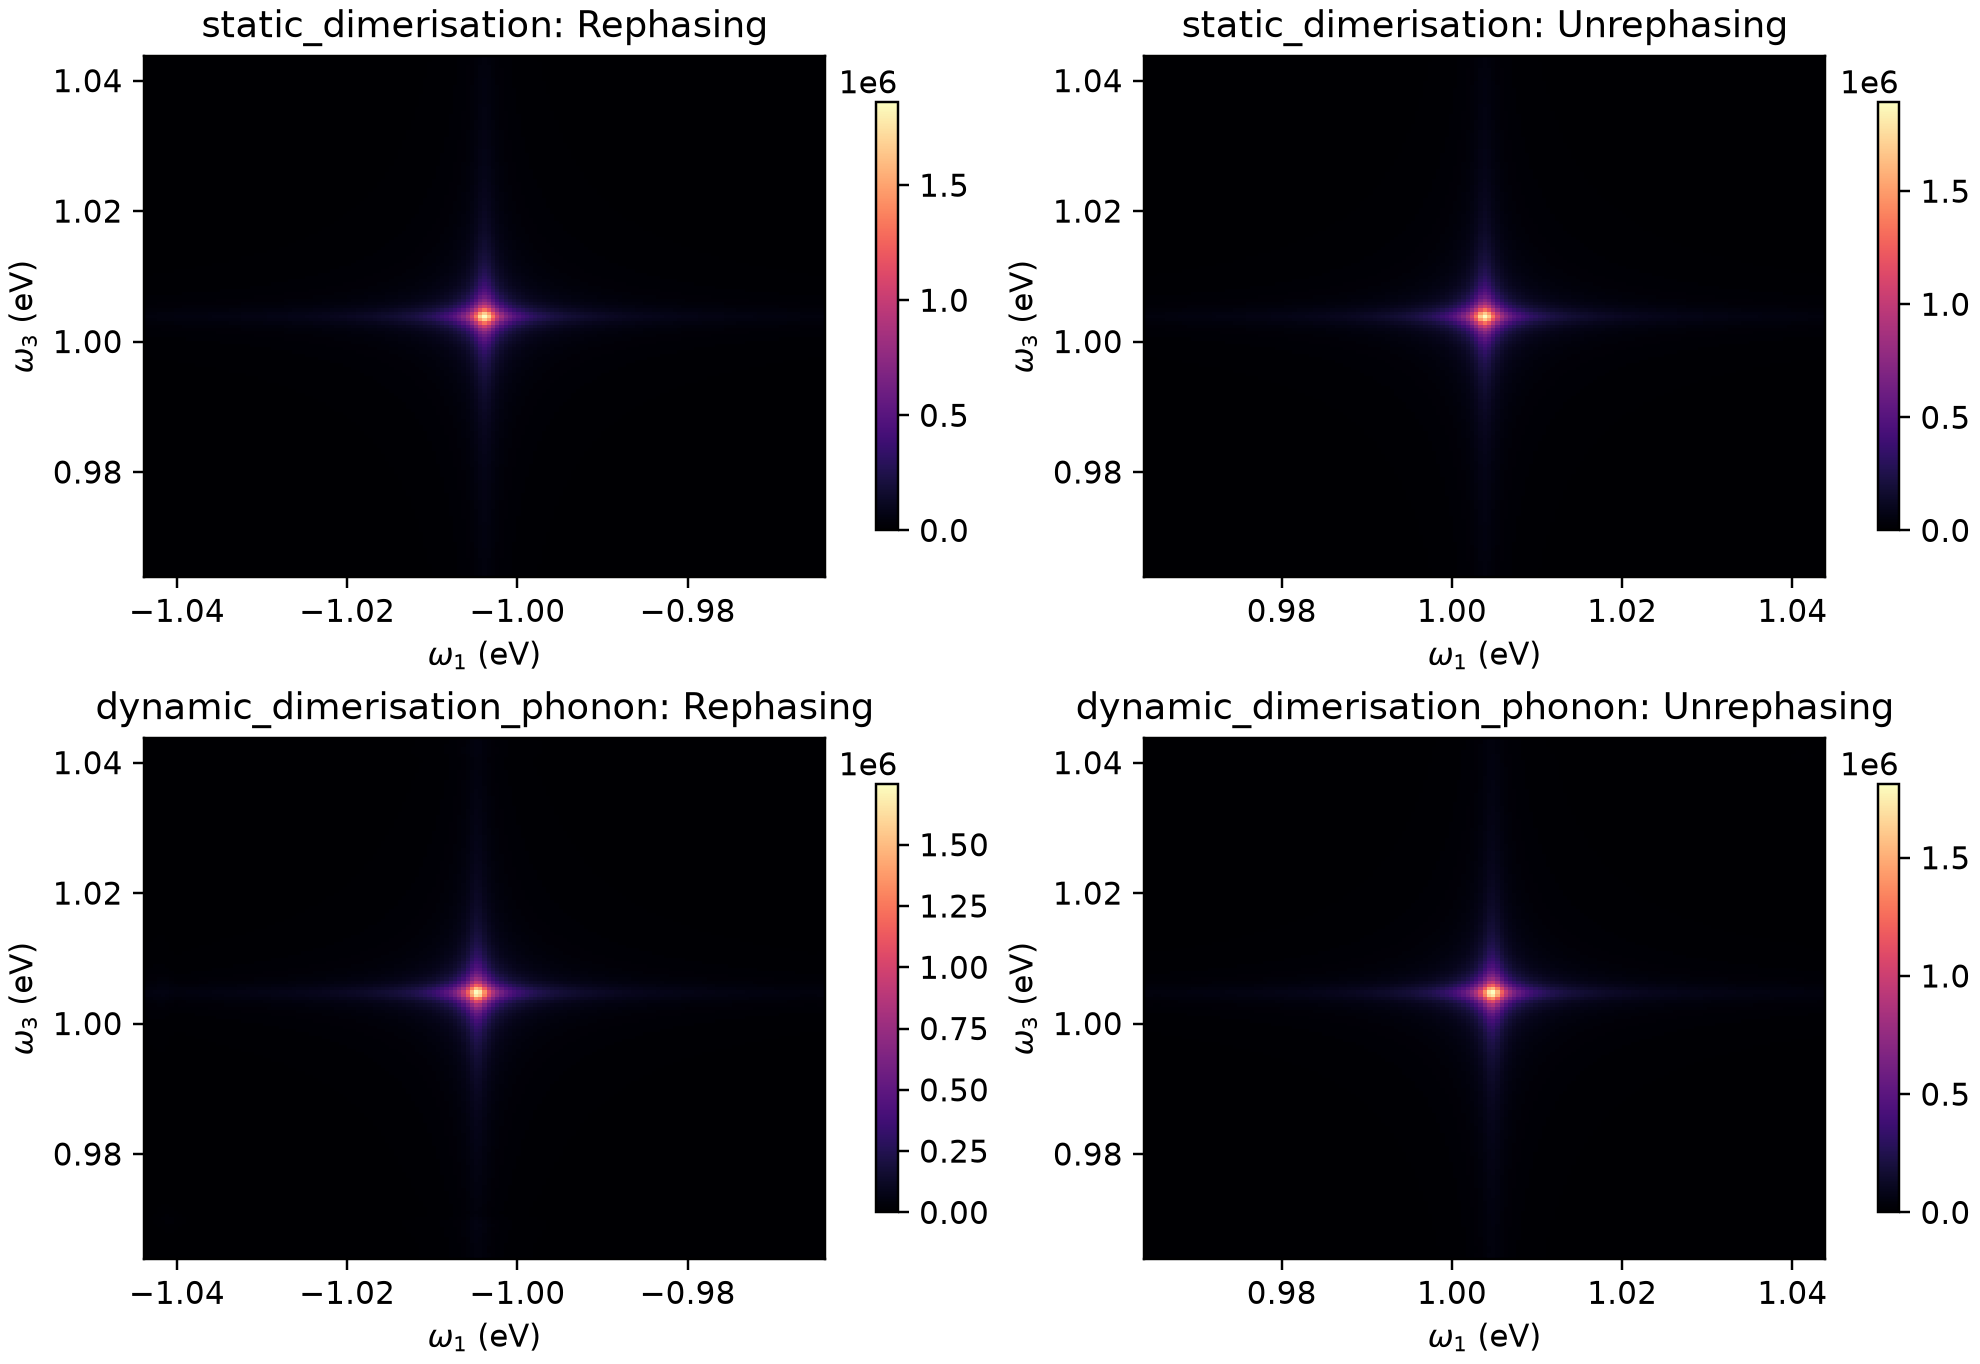
\includegraphics[width=0.98\linewidth]{spectra_etape_3_rephasing_unrephasing_abs.png}

\caption{Representative $|S|$ spectra. Left column: rephasing; right column: nonrephasing. Each panel is independently normalised.}

\end{figure}

\section{Step 5: temperature and field trends}

The nonrephasing channel checks whether the lattice-off trend above $T_{SP}$ or at high field is not a rephasing-only artefact.

\begin{table}[H]

\centering

\begin{tabular}{lrrrr}
\toprule
Case & max NR/R & $||S_{NR}||/||S_R||$ & area NR/R & NR peak $\omega_1$ \\
\midrule
T\_lattice\_T\_7 & 1.037 & 1.041 & 1.048 & 1.005 \\
T\_lattice\_T\_20 & 1.005 & 1.005 & 1.005 & 1.001 \\
T\_C1\_static\_T\_20 & 1.018 & 1.018 & 1.018 & 1.004 \\
\bottomrule
\end{tabular}

\caption{Finite-window nonrephasing ratios for Step 5: temperature and field trends.}

\end{table}

\begin{figure}[H]

\centering

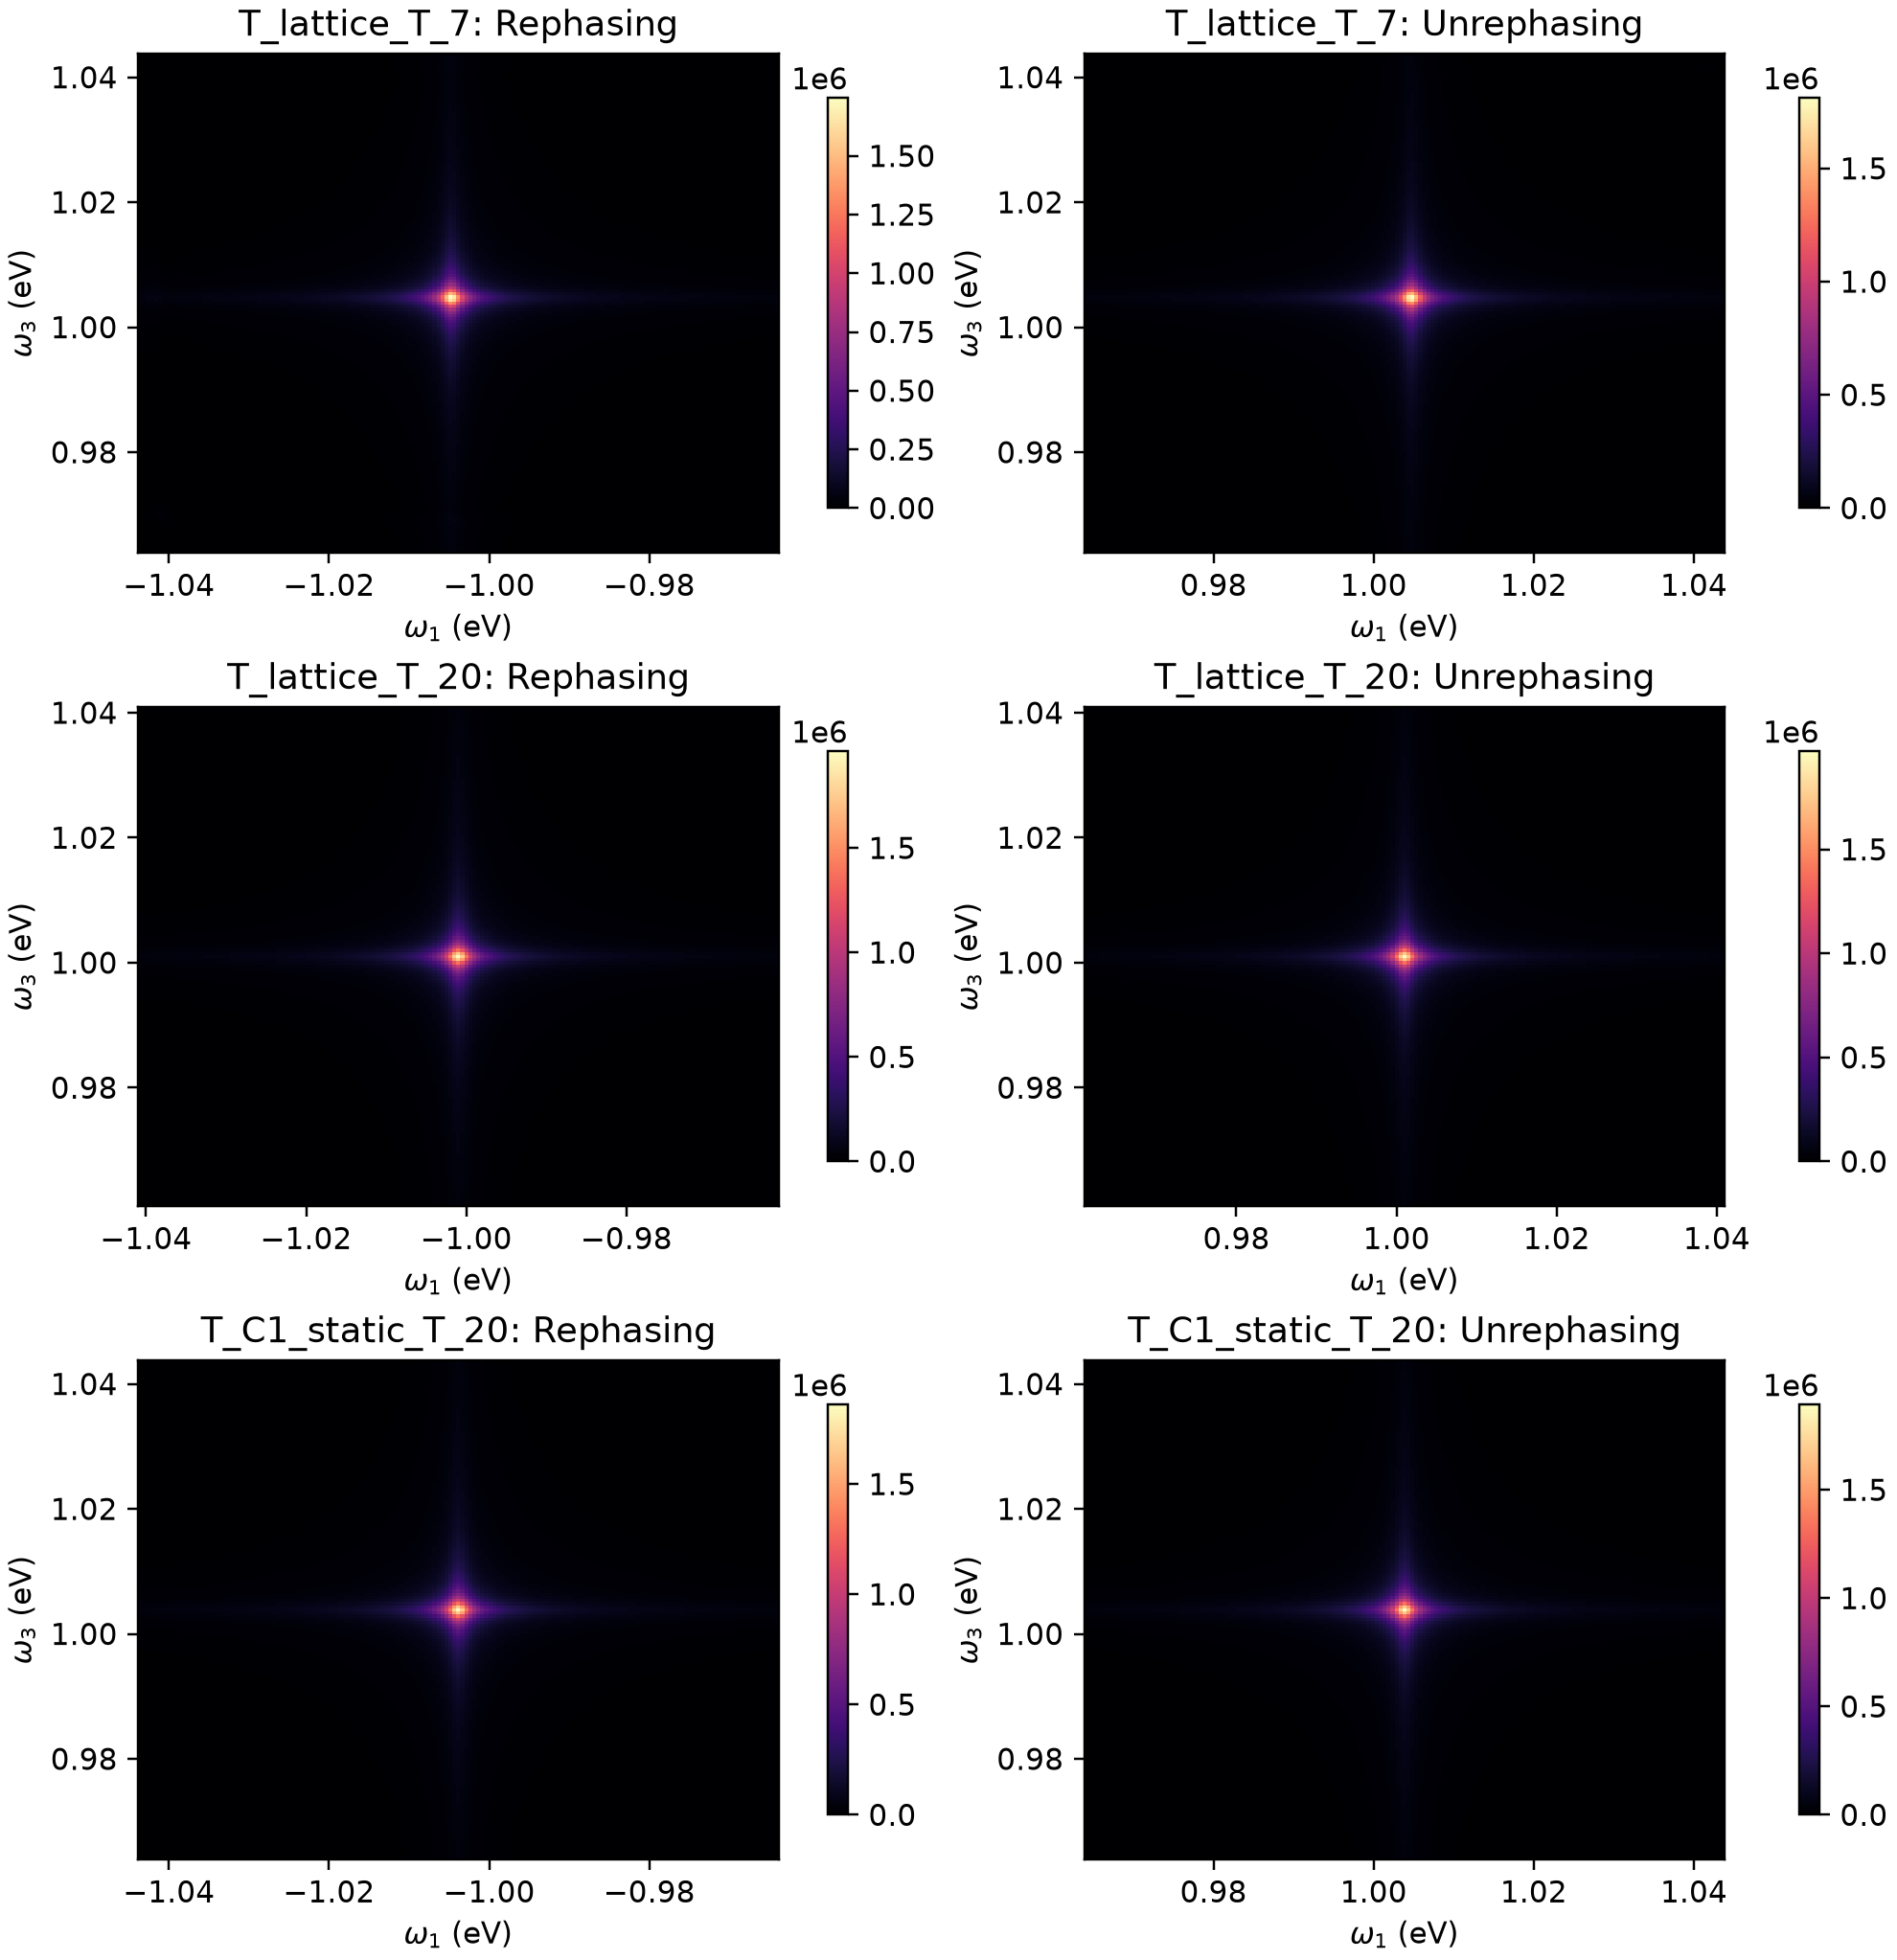
\includegraphics[width=0.98\linewidth]{spectra_etape_5_rephasing_unrephasing_abs.png}

\caption{Representative $|S|$ spectra. Left column: rephasing; right column: nonrephasing. Each panel is independently normalised.}

\end{figure}

\section{Step 2: scalar effective mixing}

This is the lower-priority scalar control: if dimerisation and local $C_1$ enter only through the same $V_{BD}^{eff}$, nonrephasing should not separate them either.

\begin{table}[H]

\centering

\begin{tabular}{lrrrr}
\toprule
Case & max NR/R & $||S_{NR}||/||S_R||$ & area NR/R & NR peak $\omega_1$ \\
\midrule
dimerisation\_control & 1.018 & 1.018 & 1.018 & 1.004 \\
spin\_correlation\_control & 1.018 & 1.018 & 1.018 & 1.004 \\
\bottomrule
\end{tabular}

\caption{Finite-window nonrephasing ratios for Step 2: scalar effective mixing.}

\end{table}

\begin{figure}[H]

\centering

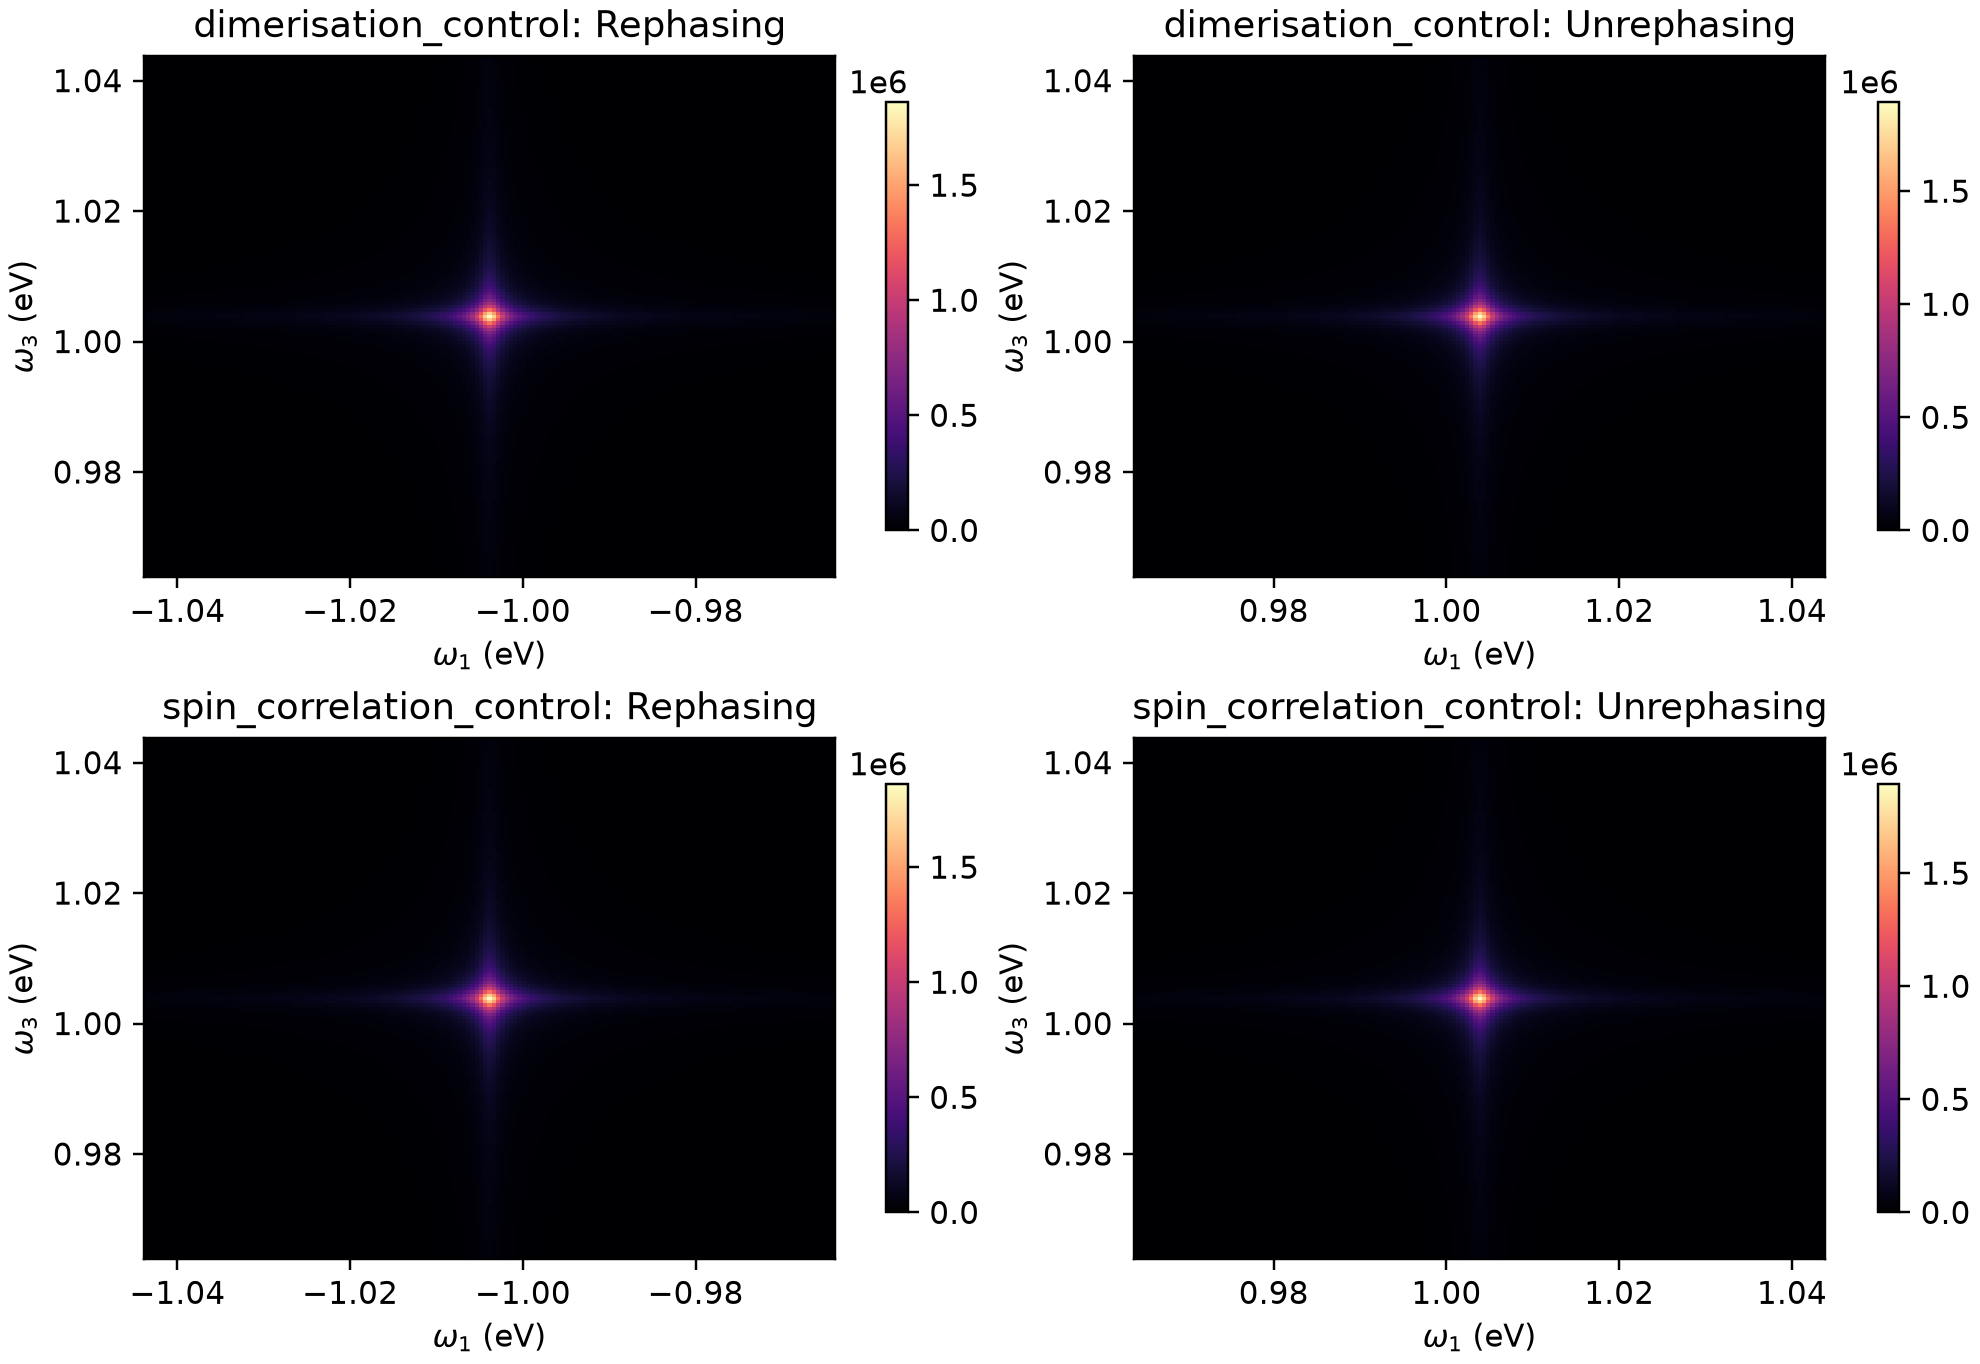
\includegraphics[width=0.98\linewidth]{spectra_etape_2_rephasing_unrephasing_abs.png}

\caption{Representative $|S|$ spectra. Left column: rephasing; right column: nonrephasing. Each panel is independently normalised.}

\end{figure}

\section{Overall conclusion}

After evaluating nonrephasing in the correct positive-coherence quadrant, the displayed nonrephasing peaks are comparable in strength to the rephasing peaks for this symmetric model.  The useful role of the nonrephasing channel is therefore not that it is a small correction, but that it provides a distinct pathway-order and quadrant check.  It confirms the scalar degeneracy of Step 2, preserves the static-control degeneracy while separating the dynamic phonon case in Step 3, and gives a corrected basis for testing the trend controls in Step 5 and the dynamic phonon scans in Step 6.

\end{document}
